\documentclass[
    titlepage,
    twoside,
    openright,
    12pt
]{book}

\usepackage{lib/polithesis}

%*****************************************************************
%                         CUSTOM PACKAGES                         
%*****************************************************************

% Should you need to add custom packages, this is the right place.

%*****************************************************************
%                      THESIS CUSTOMIZATIONS                      
%*****************************************************************
%
%   In this section, you can insert the data to be displayed in
%   the title page. If you do not want to show something, just
%   comment it using '%' at the beginning of the line.
%
%*****************************************************************

% Specify thesis language in lowercase (default "english")
\thesislanguage{english}
% Choose the font for the thesis
% The available choices are: "Computer Modern", "Baskerville",
% "Nimbus", "Palatino", "Utopia".
% If an invalid font is set, the fallback font used is the default
% LaTeX font "Computer Modern".
\thesisfont{Palatino}
% Change title color
\titlecolor{MidnightBlue}
% Change color of chapters' number
\chapnumbercolor{ThesisGray}
% The available colors are the 68 dvips colors plus the defaults.
% (https://en.wikibooks.org/wiki/LaTeX/Colors#Predefined_colors)
% You can define you own color as done for ThesisGray in the
% library file, even if it is not recommended.

%*****************************************************************
%                         TITLE PAGE DATA                         
%*****************************************************************
%
%   In this section, you can insert the data to be displayed in
%   the title page. If you do not want to show something, just
%   comment it using '%' at the beginning of the line.
%
%*****************************************************************

\university{Politecnico di Milano}
\faculty{Facoltà di Ingegneria}
\school{Scuola di Ingegneria Industriale e dell'Informazione}
\department{Dipartimento di Elettronica, Informazione e
 Bioingegneria}
\course{Computer Science and Engineering}
\title{A Fancy Title\\for a Fancy Thesis}
\supervisor{Prof. Enrico Fermi}
% You can specify more than one co-supervisor, separating them
% with commas.
\cosupervisors{Prof. Alice First, Dr. Bob Second}
% Each author should be added as a tuple of her name and her
% matriculation number joined with a comma.
% You can specify more than one author, separating each one with
% a comma. They will be printed in different lines.
\authors{Your Self, 000000, Your Second Self, 111111}
\matriculationPrefix{matr.}
\academicYear{20MM/20MN}

%*****************************************************************
%                         THESIS CONTENT                         
%*****************************************************************

\begin{document}

% Title Page
\maketitle

% Optional, comment or delete instruction to remove
\dedication{Insert here your dedication.\\Optional.}

% Chapters
\frontmatter
\pagenumbering{Roman}
\chapter{Abstract}

Nowadays, existing approaches for creating Extended Reality (XR) experiences mostly entail the use of Integrated Development Environments (IDEs) or software libraries (APIs), while the adoption of a high-level approach -- allowing to abstract from the implementation -- is however confined to technology-dependent methods or close descendants of standard meta-models.
What is needed, therefore, is a universal model that allows XR applications to be designed at the conceptual level, without relying on solutions that are domain-specific or that exclude non-programmers from designing. This thesis presents the XRM Model, a theoretical approach oriented towards the conceptualisation of XR experiences, developed from a comparative study of existing models in the literature. The XRM Model is adopted for the implementation of a High-Level Editor to support XR application designers, which was validated in a usability test with users based on the ISO 9241-11 standard. In conclusion, an experience designed for an archaeological complex was considered as a case study in order to show the benefits resulting from the adoption of the XRM and the ART Editor.


\paragraph{Keywords}  Human-Computer Interaction; Interaction Design; Extended Reality; Conceptual Modelling; Authoring tools; Tourism; Cultural Heritage
\chapter{Sommario}
Al giorno d'oggi gli approcci esistenti per la creazione di esperienze in Exted Reality (XR) consistono nella maggior parte dei casi nell'utilizzo di ambienti di sviluppo integrato (IDEs) o librerie software (APIs), mentre l'adozione di un approccio ad alto livello -- che consenta di astrarre dall'implementazione -- è tuttavia limitato a metodi dipendenti dalla tecnologia o stretti discendenti di meta-modelli standard.
È necessario, quindi, un modello universale che permetta di progettare a livello concettuale applicazioni XR, senza ricorrere a soluzioni che siano strettamente dedicate al dominio o che escludano dalla progettazione i non esperti di programmazione. In questa tesi viene presentato il Modello XRM, un approccio teorico orientato alla concettualizzazione di esperienze XR, sviluppato a partire da uno studio comparativo dei modelli esistenti in letteratura. Il Modello XRM è stato adottato per l'implementazione di un Editor ad alto livello a supporto dei designer di applicazioni XR, il quale è stato validato in un test di usabilità con utenti basato sullo standard ISO 9241-11. In conclusione si è considerato come caso di studio un'esperienza progettata per un complesso archeologico allo scopo di mostrare i benefici risultanti dall'adozione dell'XRM e dell'ART Editor.


\paragraph{Parole chiave} Human-Computer Interaction; Interaction Design; Extended Reality; Conceptual Modelling; Authoring tools; Tourism; Cultural Heritage
\chapter{Acknowledgements}

We would like to thank the company Fifthingenium S.r.l.s for the opportunity they gave us to work on this thesis project. 

Special thanks to Luigi Oliveto who supervised us during the entire project in the company. 

We would like to extend special thanks to Prof. Garzotto, and to co-supervisors Ing. Patti and Ing. Vona who supported us in the various aspects of the master thesis with great humanity, commitment and dedication.
\thesistoc

%*****************************************************************
%                            CHAPTERS                            
%*****************************************************************

\mainmatter
\chapter{Introduction}

\section{Context}
The Covid-19 pandemic situation has negatively impacted the tourism and events business sectors and thus the economy of many cities in Italy, strongly dependent on this sector.
ART (Augmented Reality for Tourism) is a project aiming at offering an innovative Extended Reality (XR) toolset to build services targeting the tourism sector, starting from the Italian market.
Thanks to solutions developed in ART, XR services and experiences will become more accessible and economically feasible, offering tourism actors a way to be more resilient to an emergency situation and safer experiences to their visitors.
Thanks to this framework, despite the current limitations regarding gatherings of people, the attractiveness of a city and its touristic points of interest will be partly supported by those actors that will invest in XR technologies, digitizing their assets and offering multiple experiences for visitors during their digital journeys, both while connecting remotely and while visiting physically.
The ART project will enhance visitors’ experience while simplifying the authoring work for the service provider. The project aims at developing a XRaaS platform, or XR as a Service, offering the opportunity to easily create multi-device XR applications starting from existing 3D models. It is mainly meant for small-medium businesses, without expertise in developing XR applications, who want to offer immersive experiences to their final customers. To achieve this, the main feature of ART will be the capability of linking the 3D content to the real world using XR helmets and a specific authoring application.

The ART project\footnote{\url{https://outoftheframe.art}} is funded by EIT Digital\footnote{\url{https://www.eitdigital.eu}} with the strategic partnership of companies as Telecom Italia (TIM) and FifthIngenium S.r.l.s.\footnote{\url{https://fifthingenium.com}} and the academic collaboration of Technische Universität Berlin (TUB) and Politecnico di Milano. This thesis is the result of the authors' work based on a company internship at Fifthingenium. 
The internship lasted 4 months during which, in a first phase, we focused on the study of XR technology and its components with the aim of designing and iteratively refining a conceptual model with all its features, and in a second phase, we contributed to the creation of an online editor designed for XR experiences.
The company also provided us with some projects, examples of real case studies that could help us define our model. 

The NURE experience is the case study used in this thesis to validate our proposal. 
NURE\footnote{\url{https://www.nurearcheologia.it}} is an organisation that was created to supply integrated services for archaeology; it is a production and work cooperative established in 2010 and based in Isili (SU), Sardinia. For almost ten years it has been involved in the management of archaeological excavations and museums, archaeological surveys, scientific assistance in restoration and conservation consolidation of monuments, preventive archaeology, cultural heritage education, museum design and layout, and the valorisation, promotion and management of archaeological sites and landscapes. 
NURE is responsible for the archaeological area of Santa Lucia di Assolo (OR), a very interesting multi-layered site that preserves important traces from the Bronze Age to the Middle Ages, with the ruins of an imposing polylobate nuraghe with its village (XIV-IX century BC), a terma, a road and several dwellings from the Imperial Roman period (III-IV century AD). There is also a Paleochristian sepulchral area with numerous tombs and a patrician funerary mausoleum located in the immediate proximity of the church, which was originally built in the Byzantine period (7th century).
In collaboration with NURE, we contributed to a Mixed Reality Musealization project of the archaeological area located in Santa Lucia di Assolo (OR), whose aim was to "revive" some very ancient archaeological sites thanks to the use of recent XR technologies.


\section{Research Questions}
An increasing trend on XR applications has been found in the last years, however literature lacks research into development of high-level design tools abstracting from the implementation, resulting mostly in tailor-made techniques. A non-technology dependant model is needed in order to allow the development of cross-reality experiences and let designers focus on relevant aspects as structural, behavioural and interaction, reducing time and resources in communication efforts within the team. At the same time, a lack of technical expertise -- usually required by traditional development environments -- prevents authors from building the experience. Therefore this work aims at answering the following research questions:
\begin{itemize}
    \item[RQ.1]\emph{What design characteristics of Extended Reality (XR) are useful, and how can they be modelled by structural, behavioral and interaction properties in a human-centered designed conceptual framework?}

    \item[RQ.2]\emph{Can a High-Level Authoring Tool facilitate the creation of XR experiences for non-expert people? What are the benefits in terms of effectiveness, efficiency and satisfaction as measured by qualitative and quantitative data?}
\end{itemize}

We answer these questions proposing an innovative and flexible conceptual model to describe XR experiences whose its submodels have the goal to define the appearance and properties of the entities -- including the user -- that structure the application, their behaviour and their resulting perceivable changes of initial properties in order to compose the activities that the user can address within the experience. In addition to this, we adapted the proposed conceptual model in the frame of the ART project guiding the development of an editor to support the authoring of XR experiences.

\section{Research Methodology}
A preliminary study of the literature allowed to understand the context and its state of the art. Several searches on the academic search engine Google Scholar have been carried out to guide the review proposed in the next chapter and structured as follows:
\begin{enumerate}
    \item A first query was related to XR and its role in tourism in the time range 2015-2020:
        \begin{itemize}
            \item \texttt{((virtual OR mixed OR augmented OR extended) AND reality) AND (cultural heritage OR tourism)}
        \end{itemize}
        After a filtering based on titles and, later on, abstracts, we selected 48 papers to review resulting in 44 useful works that guided our study.
    \item The second set of queries aimed at searching for conceptual models or modelling techniques in XR or its specifications:
        \begin{itemize}
            \item \texttt{(((design  AND methods )  OR  (conceptual  AND  (model  OR\\ models))) AND (XR  OR  MR))} in the year range 2015-2021.\\
            22 papers have been selected for further readings, that resulted in 7 relevant articles to examinate.
            \item \texttt{"conceptual modeling" OR "conceptual model" intitle:AR\\ OR intitle:"augmented reality" OR intitle:"mixed reality"} in the year range 2015-2021.\\
            Resulting in 4 works selected.
            \item \texttt{"multimodal interaction techniques" AND " ("VR" OR "AR") "} in the year range 2005-2021.\\
            10 articles found for closer examination, 2 of them have been taken in consideration for a literature review.
            \item \texttt{intitle:"modeling 3D Content" OR  intitle:"semantic\\ modeling" AND (VR OR AR OR MR)}\\
            10 articles have been selected and read, resulting in 4 relevant works accepted.
            \item Other articles have been considered based on their similarity with the topic or through citations found in the above mentioned works.
        \end{itemize}
    \item The last set of queries investigated on advances and works of the last 4 years (2018-2021) in the field of authoring tools and relevant IDEs and APIs, to offer an overview of the current platforms used in the AR/VR development field:
        \begin{itemize}
            \item \texttt{intitle:"augmented reality development" OR intitle:"AR\\ development" OR intitle:"AR framework" OR intitle:"AR\\ frameworks" OR intitle:"Augmented Reality framework" OR intitle:"AR tools" OR intitle:"Augmented Reality framework"}\\
            Starting from 113 results, only 2 papers have been chosen given the relevance with our intended research, filtering them by title, keywords and abstract.
            \item \texttt{intitle:"virtual reality development" OR intitle:"VR\\ development" OR intitle:"VR framework" OR intitle:"VR\\ frameworks" OR intitle:"Virtual Reality framework" OR intitle:"VR tools" OR intitle:"Virtual Reality framework"}\\
            Starting from 109 results, only 4 papers have been chosen given the relevance with our intended research, filtering them by title, keywords and abstract.
            \item \texttt{intitle:"authoring" OR intitle:"SDK OR SDKs" AR\\ augmented VR virtual reality}\\
            Resulting in 98 results, of which 13 papers have been selected for further reading given their relevance with the research.
            \item Other articles have been considered based on their similarity with the topic or through citations found in the above mentioned works.
        \end{itemize}
\end{enumerate}

\section{Thesis outline}
The thesis is structured as follows: \autoref{ch:background} provides an extensive review of the state of the art on XR technologies and their applications in tourism, an overview and comparative study on the existing conceptual models in XR (\autoref{sec:background-conceptual}) and, in conclusion, a thorough analysis on authoring tools in XR (\autoref{sec:background-authoring}).

The next chapter propose the XRM Conceptual Model and its sub-models: the structural (\autoref{sec:conceptual-structural}), behavioural (\autoref{sec:conceptual-behavioral}) and interaction (\autoref{sec:conceptual-interaction}) models and their application on a concrete use case (\autoref{sec:conceptual-nure-example}). 

Subsequently, \autoref{ch:art} describes the ART Framework and focuses on the implementation of the ART Editor (\autoref{sec:art-editor}) based on a high-level and low-level design process and validated on the same use case found in \autoref{sec:conceptual-nure-example} (\autoref{subsec:art-editor-nure-example}). 

An experimentation phase followed the editor design, resulting in the definition of a usability evaluation study (\autoref{ch:evaluation}) and -- consequently -- the analysis of results (\autoref{sec:evaluation-results}).

Finally, in \autoref{ch:conclusions} the concepts expressed within the thesis are summarized, and the main open challenges in the field are indicated.
\chapter{Preliminaries and State of the Art}
\label{ch:preliminaries_and_sota}

\section{Preliminary notions}
\label{sec:preliminaries}

\begin{table}[!ht]
\centering
\begin{tabular}{c l} \hline
\textbf{Notation}&\textbf{Description} \\ \hline
$G$&Graph\\
$V$&set of nodes of $G$\\
$E$&set of edges of $G$\\
$W$&set of weights corresponding to each edge in $E$\\
$w_{u,v}$&weight of edge $(u,v)$\\
$n$&$|V|$, number of nodes\\
$m$&$|E|$, number of edges\\
\hline
\end{tabular}
\caption{Graph notation.}
\label{tab:notation}
\end{table}

``In this section, we introduce the preliminary notions at the base of our study. We start by briefly introducing the problem, and then we provide the necessary concepts and the notation used."

You may insert a subsection for each of the most relevant features of your problem. You can add some reference if needed, but just to explain the problem. The references with the solutions of the problem should be put in the next section.

You can keep a notation table for the notation used in this chapter as \autoref{tab:notation}. Everything inside the notation table must be written at least once inside this chapter. You can put an extended notation for the whole thesis in the appendix.

It is likely that you have to present definitions, theorems or propositions. We suggests to use the environments provided by the template. You can find the guide in the LaTeX suggestions chapter.

\section{State of the Art}
\label{sec:sota}

In this section, we survey the most relevant works related to the argument of your thesis. If you face a problem that has more than one macro-topic, you may choose to add a subsection for each of these topics (better no more than 2-3), like \emph{Related works on Topic 1}, etc.

List the works in chronological order and cite only the most important and pertinent ones, avoid 100 citations for a master thesis.
\chapter*{\LaTeX~ suggestions}

\begin{center}
\bfseries 
\color{red}{REMOVE THIS CHAPTER BEFORE SUBMISSION}
\end{center}

\noindent In this file there are listed some tips you may find useful. Some of the shortcuts shown are custom, so I suggest you to have a look at what's next even if you are expert in LaTeX.

\section*{Math}

All the fonts supported by the template provide a math variant for the formulas. You can use the standard math commands of LaTeX plus the following additions:
\begin{itemize}
\item Argmin/max: $\argmin_i$, $\argmax_i$, and their rendering in centered equations
$$\argmin_i \quad \argmax_i$$
\item Variance: $\var$, $\Var{p}$
\item Expected value: $\ev$, $\Ev{p}$
\end{itemize}

\section*{Custom commands}

We provide two commands you may find useful.

The command \texttt{\textbackslash blankpage} adds a blank page. Differently from \texttt{\textbackslash newpage}, the added page is completely blank and the text resume from the page after.

The command \texttt{\textbackslash todo} let you add the \todo symbol in the text. You can use it whenever you have text to be revisioned after.

\section*{Environments}

The thesis package provide three useful packages you may need for the theoretical part.

\subsection*{Definition}

Definitions are used for introducing a concept and its theoretical meaning for the first time. Do not use it just for clarifying the notation. Definitions are numbered within the chapter, such that the first definition of chapter 2 is 2.1. The syntax is the following:
\begin{verbatim}
\begin{definition}[NAME (optional)]
\label{def:LABEL}
DEFINITION
\end{definition}
\end{verbatim}

\noindent Example:

\begin{definition}[$(\alpha, \beta)$-approximation]
\label{def:alphabetaapprox}
An $(\alpha, \beta)$\textit{-approximation} algorithm outputs with success probability $\beta$ a solution which is at least $\alpha$ fraction of the optimal solution, for some $\alpha, \beta \leq 1$.
\end{definition}

\subsection*{Theorem}

Theorems are numbered incrementally within the thesis, regardless of the chapter they are declared in. The syntax is the following:
\begin{verbatim}
\begin{theorem}
\label{thm:LABEL}
THEOREM
\end{theorem}
\end{verbatim}

\noindent Example:

\begin{theorem}
\label{thm:approximation}
For a non-negative, monotone, submodular function $f(\cdot)$, let $S_k$ be a set obtained by selecting $k$ elements one at a time, each time choosing an element that provides the largest marginal increase in the function value. Let $S_k^*$ be a set that maximizes the value of $f(\cdot)$ over all $k$-sized sets. Then,
$$f(S_k) \geq \left( 1-\frac{1}{e} \right) \cdot f(S_k^*).$$
\end{theorem}

\subsection*{Lemma}
Lemma are like theorems. The syntax is the following:
\begin{verbatim}
\begin{lemma}
\label{thm:LABEL}
LEMMA
\end{lemma}
\end{verbatim}

\noindent Example:

\begin{lemma}
\label{thm:lemma}
This is a lemma.
\end{lemma}

\subsection*{Proposition}
Propositions are like lemmas but they are numbered within the chapter. The syntax is the following:
\begin{verbatim}
\begin{proposition}
\label{thm:LABEL}
PROPOSITION
\end{proposition}
\end{verbatim}

\noindent Example:

\begin{proposition}
\label{thm:chernoff}
If the diffusion process starting with $S$ is simulated independently at least $r=\Omega\left(\frac{n^2}{\varepsilon^2}\ln\left(\frac{1}{\delta}\right)\right)$ times, then the average number of activated nodes over these simulations is a $(1 \pm \varepsilon)$-approximation to $\sigma(S)$, with probability at least $1 - \delta$.
\end{proposition}

\subsection*{Algorithm}
The algorithm environment is used to show pseudocodes. The syntax, which follows the same paradigm of table/tabular combo, is the following:
\begin{verbatim}
\begin{algorithm}[FLOATING OPTIONS]
\caption{CAPTION}
\label{alg:LABEL}
\begin{algorithmic}[1 if you want the lines to be numbered]
ALGORITHM
\end{algorithmic}
\end{algorithm}
\end{verbatim}

\noindent Example:

\begin{algorithm}[H]
\caption{Combinatorial Thompson Sampling}
\label{alg:cts}
\begin{algorithmic}[1]
\Require Directed graph $G(V,E)$, budget constraint $k$, time horizon $T$
\For {$i = 1$ \textbf{to} $|E|$}
\State $\alpha_i = 1, \beta_i = 1$ \Comment{Assign a Beta distribution Beta(1,1) to each edge}
\EndFor

\For {$t = 1$ \textbf{to} $T$}
\State For each arm $i$, draw a sample $\theta_i(t) \sim$ Beta$(\alpha_i, \beta_i)$
\State Let $\boldsymbol{\theta}(t) = \left(\theta_1(t), \ldots, \theta_m(t) \right)$
\State $S_t \gets$ \texttt{oracle}$(G(V,E,\boldsymbol{\theta}(t)), k)$
\State Run cascade with $S_t$ as the seed set and collect the feedback $F_t$
\State Update the Beta distributions of the edges involved using $F_t$
\EndFor
\end{algorithmic}
\end{algorithm}

\section*{Referencing}

All the declared environments above can be referenced using the \texttt{{\textbackslash autoref}} command. \autoref{def:alphabetaapprox}, \autoref{thm:approximation}, \autoref{thm:chernoff}, \autoref{alg:cts}.
\chapter{Problem formulation}
\label{ch:problem_formulation}

This chapter is dedicated to the formal presentation of the problem with the technical details. Here your should put also the figure of merit you use to compare your solution with the ones of the related works you presented.

\begin{example}
In this thesis, we address the problem of ... . [Description of the problem and classical approaches]. The figure of merit we use to compare the solutions is ... .
\end{example}

\chapter{Design and Implementation}
\label{ch:design}

``This approach is similar to the one proposed in a recent work by Nuara et al.~\cite{nuara2020driving}, in which ..."
\chapter{Experimental evaluation}
\label{ch:experiments}

This chapter shows the results of the experiments carried out to assess your contribution, usually compared to state of the art solutions. In the proposed structure, we separate experiments setup from experiment results, in which we list the experiments. This is especially convenient in case the setting is the same or very similar for all the experiments. Should this not be the case, you may consider instead to structure each experiment is a section/subsection and embed both setting and result inside it.

\begin{example}
In this chapter, we present experimental results on the algorithms proposed and we compare them with state of the art methods.
\end{example}

\section{Experimental setting}

First, describe the experimental setting. The setting usually contains:
\begin{itemize}
\item the dataset(s) used for the experiments;
\item the baselines, namely the other solutions with which you are comparing yours.
\end{itemize}

\begin{example}

\begin{table}[H]
\centering
\renewcommand{\arraystretch}{1.2}
\begin{tabular}{|l|c|c|c|c|c|}\hline
\textbf{Name}&$n$&$m$\\ \hline\hline
Email&1005&25571\\ \hline
\end{tabular}
\caption{Dataset used for the experiment.}
\label{tb:elf_datasets}
\end{table}

\paragraph{Datasets} \autoref{tb:elf_datasets} shows the characteristics of the real-world dataset used for the experiment. The dataset, provided by SNAP \cite{snapnets}, \emph{email-Eu-core}, has been generated using email data from a large European research institution. A directed edge $(u, v)$ means that person $u$ sent an e-mail to person $v$.

As widely done in literature, we assigned the ground-truth influence probabilities according to the weighted cascade model, that is, $p_{u,v}=\frac{1}{|In(v)|}$, for each edge $(u,v) \in E$.

\paragraph{Algorithms}

For the learning process, we use the Thompson Sampling (TS) as principal exploration strategy (\autoref{alg:cts}). For the sake of completeness, we show also results with a Pure Exploitation (PE) approach, in which the oracle is fed with the mean estimates of the influence probabilities at each round.

\end{example}

\section{Results}

In this section, we show and comment the results obtained from the experiments. Remember to comment every result and every figure you decide to insert in the thesis.

\begin{example}
\paragraph{Experiment 1}

\begin{figure}[H]
  \centering
  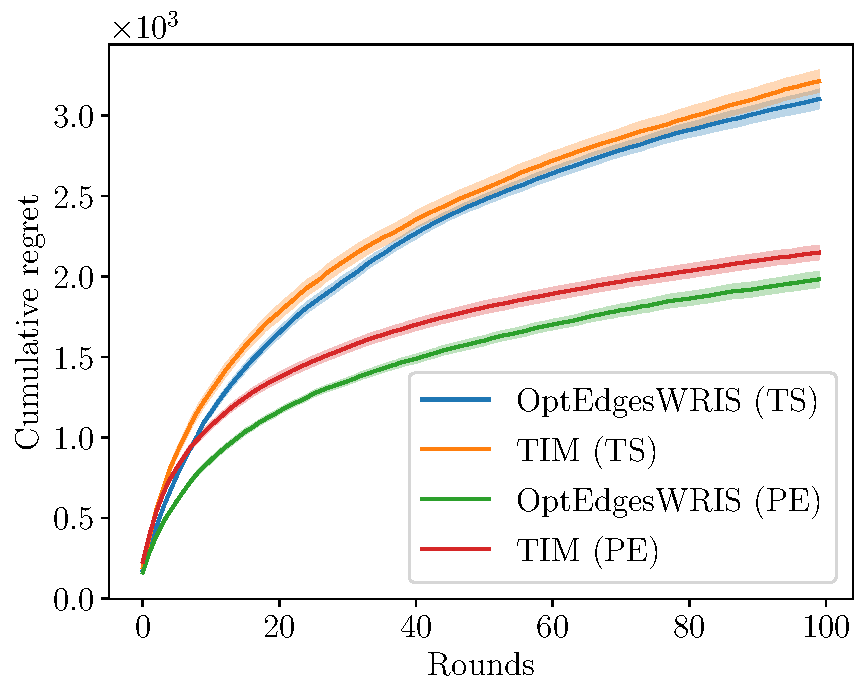
\includegraphics[width=.65\textwidth]{experiments/regret.pdf}
\caption{Cumulative regret in Email-In4 with 95\% confidence interval.}
\label{fig:exp_email}
\end{figure}

In this experiment, we test the algorithms on Email over a time horizon of $T=100$ rounds. The objective is to show the performances of the algorithms. The results have been averaged over 30 runs. \autoref{fig:exp_email} shows the cumulative regret, with a 95\% confidence interval.

As shown in the plot, our algorithm performs better with both the exploration strategies. However, the gain on TIM is more evident with the PE strategy, specially in the first rounds.
\end{example}
\chapter{Conclusions and Future Works}
\label{ch:conclusions}

In this chapter, you present the conclusions of your thesis and a couple of possible future works to extend your results. First of all, you should briefly repeat the problem you addressed in the thesis. Then, you report your achievements and how they improve the state of the art.

\section{Conclusions}
\begin{example}
In this thesis, we analyzed the problem of ... . We proposed a new approach that ... . We tested this method on ... . Reported results show that our proposal outperforms the state of the art method.
\end{example}

\section{Future works}
\begin{example}
There are several appealing paths for future works. A possible extension could be to ... .
\end{example}


%*****************************************************************
%                            APPENDIX                            
%*****************************************************************

\appendix
\chapter{Appendix}
\label{appendix}

\section{JSON State Diagram Example}
\begin{lstlisting}[caption={JSON State Diagram Example}, label=json-schema-example,basicstyle=\ttfamily\footnotesize]
{
  "ARTRecipeID": "32fcf660-7eb5-4edc-b313-e7731fc37389",
  "Name": "example",
  "Description": "Hello, world!",
  "ListOfObjects": [
    {
      "type": "2d_video",
      "id": 1
    }
  ],
  "ListOfStates": [
    {
      "Name": "state",
      "InitState": true,
      "EndState": false,
      "Objects": [
        {
          "type": "2d_video",
          "id": 1,
          "decorations": [
            {
              "type": "visibility_visible",
              "options": {
                "opacity": "100%",
                "animate": false,
                "duration": 0,
                "wait": 0
              }
            },
            {
              "type": "multimedia_pause",
              "options": {}
            }
          ]
        }
      ],
      "ListOfTransitions": [
        {
          "Name": "action",
          "Inputs": [
            {
              "type": "2d_video",
              "id": 1,
              "decorations": [
                {
                  "type": "event_tap",
                  "options": {}
                }
              ]
            }
          ],
          "NextState": "state2"
        }
      ]
    },
    {
      "Name": "state2",
      "InitState": false,
      "EndState": true,
      "Objects": [
        {
          "type": "2d_video",
          "id": 1,
          "decorations": [
            {
              "type": "multimedia_play",
              "options": {
                "loop": true
              }
            }
          ]
        }
      ],
      "ListOfTransitions": []
    }
  ]
}
\end{lstlisting}


\section{JSON State Diagram NURE Case study}
\begin{lstlisting}[caption={JSON State Diagram NURE Case study}, label=json-schema-NURE,basicstyle=\ttfamily\footnotesize]
{
  "ARTRecipeId": "88f4df4b-8bf2-4fd6-ae1e-f8fa3ec3a8b4",
  "Name": "NURE Case Study",
  "Description": "State Diagram of the NURE Experience case study.",
  "ListOfObjects": [
    {
      "type": "3d_scene",
      "id": 20
    },
    {
      "type": "3d_model",
      "id": 4
    },
    {
      "type": "3d_model",
      "id": 5
    },
    {
      "type": "3d_model",
      "id": 8
    },
    {
      "type": "3d_model",
      "id": 6
    },
    {
      "type": "3d_model",
      "id": 7
    },
    {
      "type": "3d_scene",
      "id": 10
    },
    {
      "type": "menu",
      "id": 2
    },
    {
      "type": "menu",
      "id": 3
    },
    {
      "type": "3d_scene",
      "id": 22
    },
    {
      "type": "3d_model",
      "id": 9
    },
    {
      "type": "3d_video",
      "id": 11
    },
    {
      "type": "qr_code",
      "id": 31
    },
    {
      "type": "menu",
      "id": 32
    },
    {
      "type": "3d_scene",
      "id": 30
    }
  ],
  "ListOfStates": [
    {
      "Name": "state",
      "InitState": false,
      "EndState": false,
      "Objects": [
        {
          "type": "3d_scene",
          "id": 20,
          "decorations": [
            {
              "type": "visibility_visible",
              "options": {
                "opacity": "100%",
                "animate": false,
                "duration": 0,
                "wait": 0
              }
            }
          ]
        },
        {
          "type": "3d_model",
          "id": 4,
          "decorations": [
            {
              "type": "visibility_visible",
              "options": {
                "opacity": "100%",
                "animate": false,
                "duration": 0,
                "wait": 0
              }
            },
            {
              "type": "visibility_blinking",
              "options": {
                "loop": false
              }
            }
          ]
        },
        {
          "type": "3d_model",
          "id": 5,
          "decorations": [
            {
              "type": "visibility_visible",
              "options": {
                "opacity": "100%",
                "animate": false,
                "duration": 0,
                "wait": 0
              }
            },
            {
              "type": "visibility_blinking",
              "options": {
                "loop": false
              }
            }
          ]
        },
        {
          "type": "3d_model",
          "id": 8,
          "decorations": [
            {
              "type": "visibility_visible",
              "options": {
                "opacity": "100%",
                "animate": false,
                "duration": 0,
                "wait": 0
              }
            },
            {
              "type": "visibility_blinking",
              "options": {
                "loop": false
              }
            }
          ]
        },
        {
          "type": "3d_model",
          "id": 6,
          "decorations": [
            {
              "type": "visibility_visible",
              "options": {
                "opacity": "100%",
                "animate": false,
                "duration": 0,
                "wait": 0
              }
            },
            {
              "type": "visibility_blinking",
              "options": {
                "loop": false
              }
            }
          ]
        },
        {
          "type": "3d_model",
          "id": 7,
          "decorations": [
            {
              "type": "visibility_visible",
              "options": {
                "opacity": "100%",
                "animate": false,
                "duration": 0,
                "wait": 0
              }
            },
            {
              "type": "visibility_blinking",
              "options": {
                "loop": false
              }
            }
          ]
        }
      ],
      "ListOfTransitions": [
        {
          "Name": "action",
          "ListOfInputs": [
            {
              "type": "3d_model",
              "id": 6,
              "decorations": [
                {
                  "type": "event_swipe",
                  "options": {}
                }
              ]
            }
          ],
          "NextState": "state2"
        },
        {
          "Name": "action2",
          "ListOfInputs": [
            {
              "type": "3d_model",
              "id": 7,
              "decorations": [
                {
                  "type": "event_swipe",
                  "options": {}
                }
              ]
            }
          ],
          "NextState": "state3"
        },
        {
          "Name": "action3",
          "ListOfInputs": [
            {
              "type": "3d_scene",
              "id": 20,
              "decorations": [
                {
                  "type": "event_proximity_out",
                  "options": {
                    "time": 10
                  }
                }
              ]
            }
          ],
          "NextState": "state6"
        }
      ]
    },
    {
      "Name": "state2",
      "InitState": false,
      "EndState": false,
      "Objects": [
        {
          "type": "3d_model",
          "id": 6,
          "decorations": [
            {
              "type": "visibility_hidden",
              "options": {
                "animate": false,
                "duration": 0,
                "wait": 0
              }
            }
          ]
        }
      ],
      "ListOfTransitions": [
        {
          "Name": "action2",
          "ListOfInputs": [
            {
              "type": "3d_model",
              "id": 7,
              "decorations": [
                {
                  "type": "event_swipe",
                  "options": {}
                }
              ]
            }
          ],
          "NextState": "state3"
        },
        {
          "Name": "action3",
          "ListOfInputs": [
            {
              "type": "3d_scene",
              "id": 20,
              "decorations": [
                {
                  "type": "event_proximity_out",
                  "options": {
                    "time": 10
                  }
                }
              ]
            }
          ],
          "NextState": "state6"
        }
      ]
    },
    {
      "Name": "state4",
      "InitState": true,
      "EndState": false,
      "Objects": [
        {
          "type": "3d_scene",
          "id": 10,
          "decorations": [
            {
              "type": "visibility_hidden",
              "options": {
                "animate": false,
                "duration": 0,
                "wait": 0
              }
            }
          ]
        }
      ],
      "ListOfTransitions": [
        {
          "Name": "action4",
          "ListOfInputs": [
            {
              "type": "menu",
              "id": 2,
              "decorations": [
                {
                  "type": "event_tap",
                  "options": {}
                }
              ]
            }
          ],
          "NextState": "state"
        }
      ]
    },
    {
      "Name": "state5",
      "InitState": true,
      "EndState": false,
      "Objects": [
        {
          "type": "3d_scene",
          "id": 10,
          "decorations": [
            {
              "type": "visibility_visible",
              "options": {
                "opacity": "100%",
                "animate": false,
                "duration": 0,
                "wait": 0
              }
            }
          ]
        }
      ],
      "ListOfTransitions": [
        {
          "Name": "action5",
          "ListOfInputs": [
            {
              "type": "3d_scene",
              "id": 10,
              "decorations": [
                {
                  "type": "event_proximity_out",
                  "options": {
                    "time": 10
                  }
                }
              ]
            },
            {
              "type": "3d_scene",
              "id": 20,
              "decorations": [
                {
                  "type": "event_proximity_in",
                  "options": {
                    "time": 10
                  }
                }
              ]
            }
          ],
          "NextState": "state"
        }
      ]
    },
    {
      "Name": "state3",
      "InitState": false,
      "EndState": false,
      "Objects": [
        {
          "type": "3d_model",
          "id": 7,
          "decorations": [
            {
              "type": "visibility_hidden",
              "options": {
                "animate": false,
                "duration": 0,
                "wait": 0
              }
            }
          ]
        }
      ],
      "ListOfTransitions": [
        {
          "Name": "action",
          "ListOfInputs": [
            {
              "type": "3d_model",
              "id": 6,
              "decorations": [
                {
                  "type": "event_swipe",
                  "options": {}
                }
              ]
            }
          ],
          "NextState": "state2"
        },
        {
          "Name": "action3",
          "ListOfInputs": [
            {
              "type": "3d_scene",
              "id": 20,
              "decorations": [
                {
                  "type": "event_proximity_out",
                  "options": {
                    "time": 10
                  }
                }
              ]
            }
          ],
          "NextState": "state6"
        }
      ]
    },
    {
      "Name": "state6",
      "InitState": false,
      "EndState": false,
      "Objects": [
        {
          "type": "3d_model",
          "id": 4,
          "decorations": [
            {
              "type": "visibility_hidden",
              "options": {
                "animate": false,
                "duration": 0,
                "wait": 0
              }
            }
          ]
        },
        {
          "type": "3d_model",
          "id": 5,
          "decorations": [
            {
              "type": "visibility_hidden",
              "options": {
                "animate": false,
                "duration": 0,
                "wait": 0
              }
            }
          ]
        },
        {
          "type": "3d_model",
          "id": 6,
          "decorations": [
            {
              "type": "visibility_hidden",
              "options": {
                "animate": false,
                "duration": 0,
                "wait": 0
              }
            }
          ]
        },
        {
          "type": "3d_model",
          "id": 7,
          "decorations": [
            {
              "type": "visibility_hidden",
              "options": {
                "animate": false,
                "duration": 0,
                "wait": 0
              }
            }
          ]
        }
      ],
      "ListOfTransitions": [
        {
          "Name": "action8",
          "ListOfInputs": [
            {
              "type": "menu",
              "id": 3,
              "decorations": [
                {
                  "type": "event_tap",
                  "options": {}
                }
              ]
            }
          ],
          "NextState": "state7"
        }
      ]
    },
    {
      "Name": "state7",
      "InitState": false,
      "EndState": false,
      "Objects": [
        {
          "type": "3d_scene",
          "id": 22,
          "decorations": [
            {
              "type": "visibility_visible",
              "options": {
                "opacity": "100%",
                "animate": false,
                "duration": 0,
                "wait": 0
              }
            }
          ]
        },
        {
          "type": "3d_model",
          "id": 9,
          "decorations": [
            {
              "type": "visibility_visible",
              "options": {
                "opacity": "100%",
                "animate": false,
                "duration": 0,
                "wait": 0
              }
            }
          ]
        }
      ],
      "ListOfTransitions": [
        {
          "Name": "action7",
          "ListOfInputs": [
            {
              "type": "3d_model",
              "id": 8,
              "decorations": [
                {
                  "type": "event_tap",
                  "options": {}
                }
              ]
            }
          ],
          "NextState": "state8"
        }
      ]
    },
    {
      "Name": "state8",
      "InitState": false,
      "EndState": false,
      "Objects": [
        {
          "type": "3d_model",
          "id": 9,
          "decorations": [
            {
              "type": "visibility_hidden",
              "options": {
                "animate": false,
                "duration": 0,
                "wait": 0
              }
            }
          ]
        },
        {
          "type": "3d_video",
          "id": 11,
          "decorations": [
            {
              "type": "multimedia_play",
              "options": {
                "loop": true
              }
            },
            {
              "type": "visibility_visible",
              "options": {
                "opacity": "100%",
                "animate": false,
                "duration": 0,
                "wait": 0
              }
            }
          ]
        }
      ],
      "ListOfTransitions": [
        {
          "Name": "action10",
          "ListOfInputs": [
            {
              "type": "qr_code",
              "id": 31,
              "decorations": [
                {
                  "type": "recognition_read",
                  "options": {}
                }
              ]
            }
          ],
          "NextState": "state9"
        },
        {
          "Name": "action12",
          "ListOfInputs": [
            {
              "type": "menu",
              "id": 32,
              "decorations": [
                {
                  "type": "event_tap",
                  "options": {}
                }
              ]
            }
          ],
          "NextState": "state9"
        }
      ]
    },
    {
      "Name": "state9",
      "InitState": false,
      "EndState": true,
      "Objects": [
        {
          "type": "3d_scene",
          "id": 30,
          "decorations": [
            {
              "type": "visibility_visible",
              "options": {
                "opacity": "100%",
                "animate": false,
                "duration": 0,
                "wait": 0
              }
            }
          ]
        },
        {
          "type": "3d_scene",
          "id": 22,
          "decorations": [
            {
              "type": "visibility_hidden",
              "options": {
                "animate": false,
                "duration": 0,
                "wait": 0
              }
            }
          ]
        }
      ],
      "ListOfTransitions": []
    }
  ]
}

\end{lstlisting}

\clearpage
\section{SUS Questionnaire}
\label{appendix:sus}

\newcolumntype{P}{>{\centering\arraybackslash}p{0.75cm}}
\newcolumntype{L}{>{\raggedright\arraybackslash}m{0.2\textwidth}}
\newcolumntype{R}{>{\raggedleft\arraybackslash}m{0.2\textwidth}}

\newcommand{\usetbl}{%
  \begin{tabular}{@{}|*5{P|}@{}}
    \hline
    1 & 2 & 3 & 4 & 5 \\
    \hline
  \end{tabular}
}

\newcommand\prop[1]{%
  \item
  \parbox[t]{0.5\textwidth}{#1}%
  \qquad
  \parbox[t]{0.5\textwidth}{\usetbl}%
}

\hspace*{0.625\textwidth}%
\begin{tabularx}{0.5\textwidth}{@{}LR@{}}
  \textbf{Strongly} & \textbf{Strongly} \\
  \textbf{Disagree} & \textbf{Agree} \\
\end{tabularx}
 
\begin{enumerate}
\prop{I think that I would like to use this system frequently}

\prop{I found the system unnecessarily complex}

\prop{I thought the system was easy to use}

\prop{I think that I would need the support of a technical person to be able to use this system}

\prop{I found the various functions in this system were well integrated}

\prop{I thought there was too much inconsistency in this system}

\prop{I would imagine that most people would learn to use this system very quickly}

\prop{I found the system very cumbersome to use}

\prop{I felt very confident using the system}

\prop{I needed to learn a lot of things before I could get going with this system}


\end{enumerate}


\section{Open Ended Questionnaire}
\label{appendix:openended}
\begin{enumerate}
    \item Please tell us more about what were your main problems during the use of the tool.
    \item Please tell us more about what you liked of the tool.
    \item Any further comment.
    \item Do you have some experience in Augmented Reality/Virtual Reality development?
    \item Do you have a Computer Science background?
\end{enumerate}

\section{Sub-tasks}
\label{appendix:subtasks}
\begin{longtable}{ll}
Task 1 &                              \\ \hline
\endfirsthead
%
\endhead
%
       & 3D Model placement           \\
       & Add Visible tag              \\
       & Action Node with 3D Model    \\
       & Tap Action Tag               \\
       & Link between nodes           \\
       & Linked State Node            \\
       & Add 2D Text                  \\
       & Add Visible tag              \\
       & Keep coherent IDs            \\
       &                              \\
Task 2 &                              \\ \hline
       & 2D Video placement           \\
       & Add Visible tag              \\
       & Action Node with 2D Video    \\
       & Link between nodes           \\
       & Tap Action Tag               \\
       & Final state on play          \\
       & Visible tag options          \\
       & Change label name            \\
       & On play tag options          \\
       & Keep coherent IDs            \\
       &                              \\
Task 3 &                              \\ \hline
       & Add Visible tag              \\
       & Set opacity to 90\%          \\
       & Add 2 Action Nodes           \\
       & Tap Action Tag               \\
       & Final state on play          \\
       & Add Proximity Out tag        \\
       & Link the action backwards    \\
       & Proximity Out tag options    \\
       & On play tag loop option      \\
       & Keep coherent IDs            \\
       &                              \\
Task 4 &                              \\ \hline
       & Change recipe name           \\
       & Add Audio off tag            \\
       & Add Subtitles on tag         \\
       & Add 3D Model                 \\
       & Add 3D Video                 \\
       & Add Proximity Out action tag \\
       & Add Proximity In action tag  \\
       & Add Blink tag                \\
       & Add Hidden tag               \\
       & Keep coherent IDs            \\
       & Save the experience         
\end{longtable}
\chapter*{Acknowledgments}
Here you can insert optionally the acknowledgments for who had a significant importance for the accomplishment of this goal. These acknowledgments are less formal than the ones at the beginning of the thesis and are not listed in the table of contents.

%*****************************************************************
%                         REFERENCE LIST                         
%*****************************************************************

\bibliography{biblio}

\end{document}